\documentclass{article}
\usepackage[T1]{fontenc}
\usepackage{lmodern}
\usepackage[utf8]{inputenc}
\usepackage{amsmath,amssymb,amsfonts,amsthm}
\usepackage{graphicx}
\usepackage{geometry}
\usepackage{tcolorbox}
\usepackage{hyperref}
\usepackage{float}

\geometry{margin=1in}

\title{\textbf{CBSE Class 12 Mathematics (Delhi 2008)}\\\large Solutions and Computational Verification Manual}
\author{\textbf{G. V. V. Sharma} \\ Department of Electrical Engineering \\ Indian Institute of Technology Hyderabad}
\date{November 2026}

\begin{document}

\maketitle

\section*{ABOUT THIS DOCUMENT}
This document provides complete step-by-step analytical solutions to the CBSE Class 12 Mathematics 2008 Delhi Board Examination (29 questions across Sections A, B, and C). In accordance with modern scientific computing paradigms:
\begin{enumerate}
    \item Each question is accompanied by theoretical derivations cross-referenced to standard formulae in Section 1.1.
    \item Differential equations are solved strictly using \textbf{Laplace transform} methods.
    \item Vector magnitude problems are solved using the rigorous \textbf{norm of vector} ($\|\mathbf{v}\| = \sqrt{\mathbf{v}^\top \mathbf{v}}$) formulation.
    \item Every problem includes verified \textbf{C} or \textbf{Python} scripts located in the \texttt{codes/} directory, designed for compilation and execution in mobile Linux environments such as Termux.
    \item Geometric and analytical curves are plotted with Matplotlib and saved directly as raster figures for inspection.
\end{enumerate}

\newpage
\tableofcontents
\newpage

\section{CBSE Class 12 Mathematics 2008}

\subsection{Formulae}

\begin{align}
\intertext{\textbf{1.1.1 Probability Rules}}
& \Pr(A + B) = \Pr(A) + \Pr(B) - \Pr(AB) \label{eq:prob_union} \\
& \Pr(A|B) = \frac{\Pr(AB)}{\Pr(B)} \label{eq:prob_cond} \\
& \Pr(E_i|A) = \frac{\Pr(E_i)\Pr(A|E_i)}{\sum_{k=1}^n \Pr(E_k)\Pr(A|E_k)} \quad \text{(Bayes' Theorem)} \label{eq:bayes} \\
& P(X = r) = \binom{n}{r} p^r q^{n-r}, \quad q = 1 - p \quad \text{(Binomial Distribution)} \label{eq:binomial}
\end{align}

\begin{align}
\intertext{\textbf{1.1.2 Laplace Transforms for Differential Equations}}
& \mathcal{L}\{y(t)\} = Y(s) = \int_0^\infty e^{-st} y(t) \, dt \label{eq:laplace_def} \\
& \mathcal{L}\{y'(t)\} = s Y(s) - y(0) \label{eq:laplace_first_deriv} \\
& \mathcal{L}\{y''(t)\} = s^2 Y(s) - s y(0) - y'(0) \label{eq:laplace_second_deriv} \\
& \mathcal{L}\{t^n\} = \frac{n!}{s^{n+1}}, \quad \mathcal{L}\{e^{at}\} = \frac{1}{s - a} \label{eq:laplace_powers} \\
& \mathcal{L}^{-1}\left\{\frac{1}{(s+a)^2}\right\} = t e^{-at} \label{eq:laplace_shift}
\end{align}

\begin{align}
\intertext{\textbf{1.1.3 Vectors and Norm Procedure}}
& \|\mathbf{a}\| = \sqrt{\mathbf{a}^\top \mathbf{a}} = \sqrt{a_1^2 + a_2^2 + a_3^2} \label{eq:vector_norm} \\
& \hat{\mathbf{a}} = \frac{\mathbf{a}}{\|\mathbf{a}\|} \label{eq:unit_vector} \\
& \cos \theta = \frac{\mathbf{a}^\top \mathbf{b}}{\|\mathbf{a}\| \|\mathbf{b}\|} \label{eq:angle_between} \\
& \mathbf{a} \times \mathbf{b} = \begin{vmatrix} \hat{i} & \hat{j} & \hat{k} \\ a_1 & a_2 & a_3 \\ b_1 & b_2 & b_3 \end{vmatrix} \label{eq:cross_prod} \\
& d = \frac{|(\mathbf{a}_2 - \mathbf{a}_1)^\top (\mathbf{b}_1 \times \mathbf{b}_2)|}{\|\mathbf{b}_1 \times \mathbf{b}_2\|} \quad \text{(Shortest distance between skew lines)} \label{eq:shortest_dist}
\end{align}

\begin{align}
\intertext{\textbf{1.1.4 Matrices and Determinants}}
& A = \frac{1}{2}(A + A^\top) + \frac{1}{2}(A - A^\top) \label{eq:matrix_decomp} \\
& \det(AB) = \det(A)\det(B), \quad \det(A^\top) = \det(A) \label{eq:det_props} \\
& C_{ij} = (-1)^{i+j} M_{ij} \label{eq:cofactor}
\end{align}

\begin{align}
\intertext{\textbf{1.1.5 Calculus and Trigonometry}}
& \tan^{-1} x + \tan^{-1} y = \tan^{-1}\left(\frac{x+y}{1 - xy}\right), \quad xy < 1 \label{eq:arctan_sum} \\
& \int \frac{f'(x)}{f(x)} \, dx = \ln|f(x)| + C \label{eq:log_integral} \\
& \int_0^a f(x) \, dx = \int_0^a f(a - x) \, dx \label{eq:def_integral_prop}
\end{align}

\newpage
\subsection{Problems and Solutions}

\subsubsection*{Section A (1 Mark Each)}

\paragraph{1.2.1 Question 1}
If $f(x) = x + 7$ and $g(x) = x - 7$, $x \in \mathbb{R}$, find $(f \circ g)(7)$.

\textbf{Solution:} By definition of composite functions,
\begin{equation}
(f \circ g)(x) = f(g(x))
\end{equation}
Evaluating at $x = 7$:
\begin{align}
g(7) &= 7 - 7 = 0 \\
f(g(7)) &= f(0) = 0 + 7 = 7
\end{align}
Hence, $(f \circ g)(7) = 7$.
\begin{tcolorbox}[colback=gray!10,colframe=black,width=\linewidth]
\texttt{codes/q01.c}
\end{tcolorbox}

\paragraph{1.2.2 Question 2}
Evaluate: $\sin\left[\frac{\pi}{3} - \sin^{-1}\left(-\frac{1}{2}\right)\right]$.

\textbf{Solution:} Since $\sin^{-1}(-x) = -\sin^{-1}(x)$, we have:
\begin{equation}
\sin^{-1}\left(-\frac{1}{2}\right) = -\frac{\pi}{6}
\end{equation}
Substituting this value into the expression:
\begin{align}
\sin\left[\frac{\pi}{3} - \left(-\frac{\pi}{6}\right)\right] &= \sin\left(\frac{\pi}{3} + \frac{\pi}{6}\right) = \sin\left(\frac{\pi}{2}\right) = 1
\end{align}
\begin{tcolorbox}[colback=gray!10,colframe=black,width=\linewidth]
\texttt{codes/q02.c}
\end{tcolorbox}

\paragraph{1.2.3 Question 3}
Find the value of $x$ and $y$ if:
\begin{equation}
2\begin{pmatrix} 1 & 3 \\ 0 & x \end{pmatrix} + \begin{pmatrix} y & 0 \\ 1 & 2 \end{pmatrix} = \begin{pmatrix} 5 & 6 \\ 1 & 8 \end{pmatrix}
\end{equation}

\textbf{Solution:} Performing scalar multiplication and matrix addition:
\begin{equation}
\begin{pmatrix} 2 & 6 \\ 0 & 2x \end{pmatrix} + \begin{pmatrix} y & 0 \\ 1 & 2 \end{pmatrix} = \begin{pmatrix} 2+y & 6 \\ 1 & 2x+2 \end{pmatrix} = \begin{pmatrix} 5 & 6 \\ 1 & 8 \end{pmatrix}
\end{equation}
Equating corresponding entries:
\begin{align}
2 + y &= 5 \implies y = 3 \\
2x + 2 &= 8 \implies 2x = 6 \implies x = 3
\end{align}
Thus, $x = 3$ and $y = 3$.
\begin{tcolorbox}[colback=gray!10,colframe=black,width=\linewidth]
\texttt{codes/q03.c}
\end{tcolorbox}

\paragraph{1.2.4 Question 4}
Evaluate:
\begin{equation}
\begin{vmatrix} a + ib & c + id \\ -c + id & a - ib \end{vmatrix}
\end{equation}

\textbf{Solution:} Expanding the $2 \times 2$ determinant:
\begin{align}
\Delta &= (a + ib)(a - ib) - (c + id)(-c + id) \\
&= (a^2 - i^2 b^2) - (-(c^2 - i^2 d^2)) \\
&= (a^2 + b^2) - (-(c^2 + d^2)) = a^2 + b^2 + c^2 + d^2
\end{align}
\begin{tcolorbox}[colback=gray!10,colframe=black,width=\linewidth]
\texttt{codes/q04.c}
\end{tcolorbox}

\paragraph{1.2.5 Question 5}
Find the co-factor of $a_{12}$ in the determinant:
\begin{equation}
\begin{vmatrix} 2 & -3 & 5 \\ 6 & 0 & 4 \\ 1 & 5 & -7 \end{vmatrix}
\end{equation}

\textbf{Solution:} From formula \eqref{eq:cofactor}, the cofactor $C_{12}$ is given by:
\begin{align}
C_{12} &= (-1)^{1+2} M_{12} = -\begin{vmatrix} 6 & 4 \\ 1 & -7 \end{vmatrix} \\
&= -(6(-7) - 4(1)) = -(-42 - 4) = -(-46) = 46
\end{align}
\begin{tcolorbox}[colback=gray!10,colframe=black,width=\linewidth]
\texttt{codes/q05.c}
\end{tcolorbox}

\paragraph{1.2.6 Question 6}
Evaluate:
\begin{equation}
\int \frac{x^2}{1 + x^3} \, dx
\end{equation}

\textbf{Solution:} Let $t = 1 + x^3$. Then $dt = 3x^2 dx$, which implies $x^2 dx = \frac{1}{3} dt$. From \eqref{eq:log_integral}:
\begin{equation}
\int \frac{x^2}{1 + x^3} \, dx = \frac{1}{3} \int \frac{dt}{t} = \frac{1}{3}\ln|t| + C = \frac{1}{3}\ln|1 + x^3| + C
\end{equation}
\begin{tcolorbox}[colback=gray!10,colframe=black,width=\linewidth]
\texttt{codes/q06.py}
\end{tcolorbox}

\paragraph{1.2.7 Question 7}
Evaluate:
\begin{equation}
\int_0^1 \frac{dx}{1 + x^2}
\end{equation}

\textbf{Solution:} Using the standard integral $\int \frac{dx}{1 + x^2} = \tan^{-1} x$:
\begin{equation}
\int_0^1 \frac{dx}{1 + x^2} = \left[ \tan^{-1} x \right]_0^1 = \tan^{-1}(1) - \tan^{-1}(0) = \frac{\pi}{4} - 0 = \frac{\pi}{4}
\end{equation}
\begin{tcolorbox}[colback=gray!10,colframe=black,width=\linewidth]
\texttt{codes/q07.c}
\end{tcolorbox}

\paragraph{1.2.8 Question 8}
Find a unit vector in the direction of $\mathbf{a} = 3\hat{i} + 2\hat{j} + 6\hat{k}$.

\textbf{Solution:} From formula \eqref{eq:vector_norm}, we evaluate the norm:
\begin{equation}
\|\mathbf{a}\| = \sqrt{\mathbf{a}^\top \mathbf{a}} = \sqrt{3^2 + 2^2 + 6^2} = \sqrt{9 + 4 + 36} = \sqrt{49} = 7
\end{equation}
From formula \eqref{eq:unit_vector}, the unit vector is:
\begin{equation}
\hat{\mathbf{a}} = \frac{\mathbf{a}}{\|\mathbf{a}\|} = \frac{3\hat{i} + 2\hat{j} + 6\hat{k}}{7} = \frac{3}{7}\hat{i} + \frac{2}{7}\hat{j} + \frac{6}{7}\hat{k}
\end{equation}
\begin{tcolorbox}[colback=gray!10,colframe=black,width=\linewidth]
\texttt{codes/q08.c}
\end{tcolorbox}

\paragraph{1.2.9 Question 9}
Find the angle between the vectors $\mathbf{a} = \hat{i} - 2\hat{j} + 3\hat{k}$ and $\mathbf{b} = 3\hat{i} - 2\hat{j} + \hat{k}$.

\textbf{Solution:} From formula \eqref{eq:vector_norm}, compute the norms:
\begin{align}
\|\mathbf{a}\| &= \sqrt{1^2 + (-2)^2 + 3^2} = \sqrt{1 + 4 + 9} = \sqrt{14} \\
\|\mathbf{b}\| &= \sqrt{3^2 + (-2)^2 + 1^2} = \sqrt{9 + 4 + 1} = \sqrt{14}
\end{align}
The inner product is:
\begin{equation}
\mathbf{a}^\top \mathbf{b} = (1)(3) + (-2)(-2) + (3)(1) = 3 + 4 + 3 = 10
\end{equation}
From formula \eqref{eq:angle_between}:
\begin{equation}
\cos \theta = \frac{\mathbf{a}^\top \mathbf{b}}{\|\mathbf{a}\| \|\mathbf{b}\|} = \frac{10}{\sqrt{14}\sqrt{14}} = \frac{10}{14} = \frac{5}{7} \implies \theta = \cos^{-1}\left(\frac{5}{7}\right)
\end{equation}
\begin{tcolorbox}[colback=gray!10,colframe=black,width=\linewidth]
\texttt{codes/q09.c}
\end{tcolorbox}

\paragraph{1.2.10 Question 10}
For what value of $\lambda$ are the vectors $\mathbf{a} = 2\hat{i} + \lambda\hat{j} + \hat{k}$ and $\mathbf{b} = \hat{i} - 2\hat{j} + 3\hat{k}$ perpendicular to each other?

\textbf{Solution:} Two vectors are orthogonal if and only if their inner product is zero:
\begin{align}
\mathbf{a}^\top \mathbf{b} = 0 &\implies (2)(1) + (\lambda)(-2) + (1)(3) = 0 \\
&\implies 2 - 2\lambda + 3 = 0 \implies 5 - 2\lambda = 0 \implies \lambda = \frac{5}{2}
\end{align}
\begin{tcolorbox}[colback=gray!10,colframe=black,width=\linewidth]
\texttt{codes/q10.c}
\end{tcolorbox}

\newpage
\subsubsection*{Section B (4 Marks Each)}

\paragraph{1.2.11 Question 11}
Is the binary operation $*$ defined on $\mathbb{Q}$ by $a * b = \frac{a + b}{2}$ commutative? Is it associative?

\textbf{Solution:}
\begin{enumerate}
    \item \textbf{Commutativity:} For all $a, b \in \mathbb{Q}$:
    \begin{equation}
    b * a = \frac{b + a}{2} = \frac{a + b}{2} = a * b
    \end{equation}
    Hence, $*$ is commutative.
    \item \textbf{Associativity:} Consider three elements $a, b, c \in \mathbb{Q}$:
    \begin{align}
    (a * b) * c &= \left(\frac{a + b}{2}\right) * c = \frac{\frac{a + b}{2} + c}{2} = \frac{a + b + 2c}{4} \\
    a * (b * c) &= a * \left(\frac{b + c}{2}\right) = \frac{a + \frac{b + c}{2}}{2} = \frac{2a + b + c}{4}
    \end{align}
    Since $(a * b) * c \neq a * (b * c)$ in general, $*$ is not associative.
\end{enumerate}
\begin{tcolorbox}[colback=gray!10,colframe=black,width=\linewidth]
\texttt{codes/q11.c}
\end{tcolorbox}

\paragraph{1.2.12 Question 12}
Prove that:
\begin{equation}
\tan^{-1}\frac{1}{3} + \tan^{-1}\frac{1}{5} + \tan^{-1}\frac{1}{7} + \tan^{-1}\frac{1}{8} = \frac{\pi}{4}
\end{equation}

\textbf{Solution:} Applying formula \eqref{eq:arctan_sum} pair-wise:
\begin{align}
\tan^{-1}\frac{1}{3} + \tan^{-1}\frac{1}{5} &= \tan^{-1}\left(\frac{\frac{1}{3} + \frac{1}{5}}{1 - \frac{1}{15}}\right) = \tan^{-1}\left(\frac{8/15}{14/15}\right) = \tan^{-1}\left(\frac{4}{7}\right) \\
\tan^{-1}\frac{1}{7} + \tan^{-1}\frac{1}{8} &= \tan^{-1}\left(\frac{\frac{1}{7} + \frac{1}{8}}{1 - \frac{1}{56}}\right) = \tan^{-1}\left(\frac{15/56}{55/56}\right) = \tan^{-1}\left(\frac{3}{11}\right)
\end{align}
Combining both results:
\begin{align}
\tan^{-1}\left(\frac{4}{7}\right) + \tan^{-1}\left(\frac{3}{11}\right) &= \tan^{-1}\left(\frac{\frac{4}{7} + \frac{3}{11}}{1 - \frac{12}{77}}\right) = \tan^{-1}\left(\frac{\frac{44 + 21}{77}}{\frac{77 - 12}{77}}\right) = \tan^{-1}\left(\frac{65}{65}\right) = \tan^{-1}(1) = \frac{\pi}{4}
\end{align}
\begin{tcolorbox}[colback=gray!10,colframe=black,width=\linewidth]
\texttt{codes/q12.c}
\end{tcolorbox}

\paragraph{1.2.13 Question 13}
Let $A = \begin{pmatrix} 3 & 4 & 5 \\ 4 & 4 & 3 \\ 0 & 4 & 7 \end{pmatrix}$. Express $A$ as the sum of a symmetric and a skew-symmetric matrix.

\textbf{Solution:} From formula \eqref{eq:matrix_decomp}, $A = P + Q$ where $P = \frac{1}{2}(A + A^\top)$ is symmetric and $Q = \frac{1}{2}(A - A^\top)$ is skew-symmetric.
\begin{align}
A^\top &= \begin{pmatrix} 3 & 4 & 0 \\ 4 & 4 & 4 \\ 5 & 3 & 7 \end{pmatrix} \\
P &= \frac{1}{2}\begin{pmatrix} 6 & 8 & 5 \\ 8 & 8 & 7 \\ 5 & 7 & 14 \end{pmatrix} = \begin{pmatrix} 3 & 4 & 2.5 \\ 4 & 4 & 3.5 \\ 2.5 & 3.5 & 7 \end{pmatrix} \\
Q &= \frac{1}{2}\begin{pmatrix} 0 & 0 & 5 \\ 0 & 0 & -1 \\ -5 & 1 & 0 \end{pmatrix} = \begin{pmatrix} 0 & 0 & 2.5 \\ 0 & 0 & -0.5 \\ -2.5 & 0.5 & 0 \end{pmatrix}
\end{align}
Clearly $P^\top = P$, $Q^\top = -Q$, and $P + Q = A$.
\begin{tcolorbox}[colback=gray!10,colframe=black,width=\linewidth]
\texttt{codes/q13.c}
\end{tcolorbox}

\paragraph{1.2.14 Question 14}
For what value of $k$ is the following function continuous at $x = 2$?
\begin{equation}
f(x) = \begin{cases} 2x + 1, & x < 2 \\ k, & x = 2 \\ 3x - 1, & x > 2 \end{cases}
\end{equation}

\textbf{Solution:} For continuity at $x = 2$, $\lim_{x \to 2^-} f(x) = \lim_{x \to 2^+} f(x) = f(2)$.
\begin{align}
\lim_{x \to 2^-} f(x) &= \lim_{x \to 2^-} (2x + 1) = 2(2) + 1 = 5 \\
\lim_{x \to 2^+} f(x) &= \lim_{x \to 2^+} (3x - 1) = 3(2) - 1 = 5 \\
f(2) &= k
\end{align}
Therefore, $k = 5$.
\begin{figure}[H]
\centering
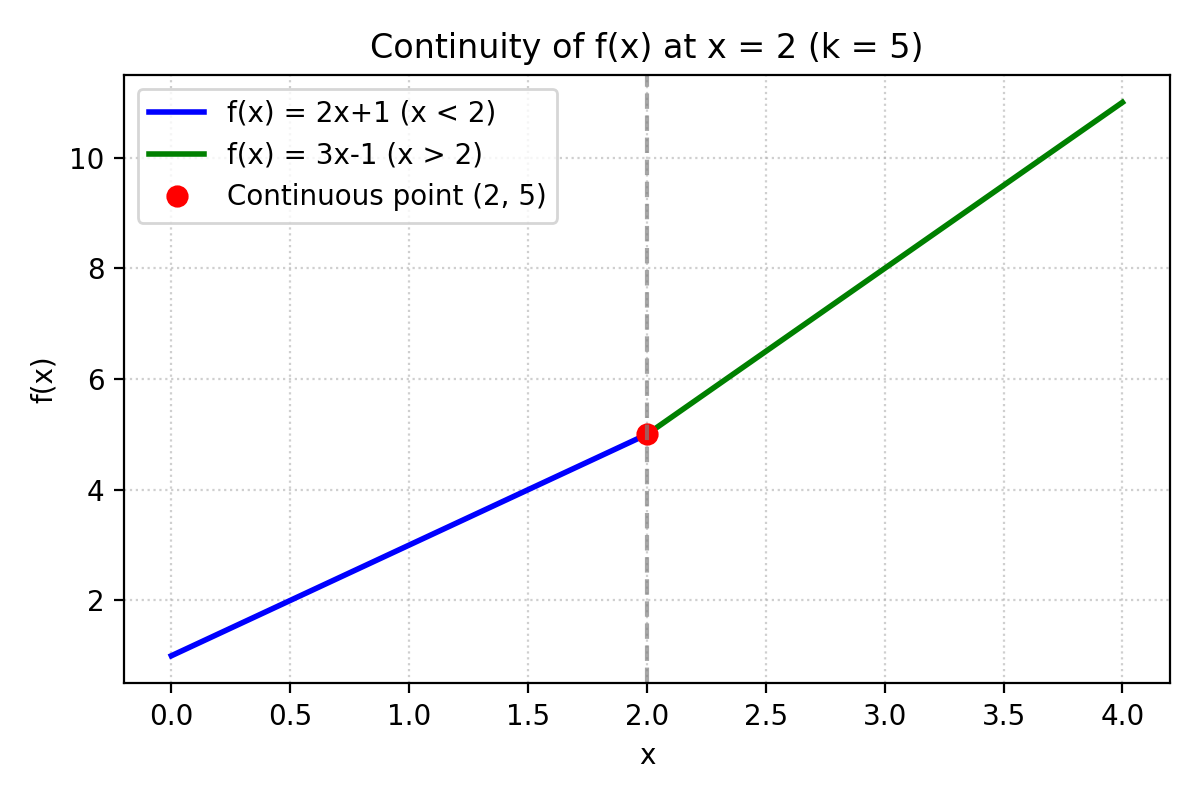
\includegraphics[width=0.65\linewidth]{figs/q14_continuity.png}
\caption{Continuity of $f(x)$ at $x = 2$ for $k = 5$.}
\end{figure}
\begin{tcolorbox}[colback=gray!10,colframe=black,width=\linewidth]
\texttt{codes/q14.py}
\end{tcolorbox}

\paragraph{1.2.15 Question 15}
Differentiate with respect to $x$:
\begin{equation}
y = \tan^{-1}\left(\frac{\sqrt{1+x} - \sqrt{1-x}}{\sqrt{1+x} + \sqrt{1-x}}\right)
\end{equation}

\textbf{Solution:} Substitute $x = \cos 2\theta$, so $\theta = \frac{1}{2}\cos^{-1} x$.
\begin{align}
\sqrt{1 + x} &= \sqrt{1 + \cos 2\theta} = \sqrt{2\cos^2\theta} = \sqrt{2}\cos\theta \\
\sqrt{1 - x} &= \sqrt{1 - \cos 2\theta} = \sqrt{2\sin^2\theta} = \sqrt{2}\sin\theta
\end{align}
Substituting into $y$:
\begin{align}
y &= \tan^{-1}\left(\frac{\sqrt{2}\cos\theta - \sqrt{2}\sin\theta}{\sqrt{2}\cos\theta + \sqrt{2}\sin\theta}\right) = \tan^{-1}\left(\frac{1 - \tan\theta}{1 + \tan\theta}\right) \\
&= \tan^{-1}\left(\tan\left(\frac{\pi}{4} - \theta\right)\right) = \frac{\pi}{4} - \theta = \frac{\pi}{4} - \frac{1}{2}\cos^{-1} x
\end{align}
Differentiating with respect to $x$:
\begin{equation}
\frac{dy}{dx} = -\frac{1}{2}\left(-\frac{1}{\sqrt{1 - x^2}}\right) = \frac{1}{2\sqrt{1 - x^2}}
\end{equation}
\begin{tcolorbox}[colback=gray!10,colframe=black,width=\linewidth]
\texttt{codes/q15.py}
\end{tcolorbox}

\paragraph{1.2.16 Question 16}
Find the equation of the tangent to the curve $x = \sin 3t$, $y = \cos 2t$ at $t = \frac{\pi}{4}$.

\textbf{Solution:} At $t = \frac{\pi}{4}$:
\begin{align}
x_0 &= \sin\left(\frac{3\pi}{4}\right) = \frac{1}{\sqrt{2}}, \quad y_0 = \cos\left(\frac{2\pi}{4}\right) = \cos\left(\frac{\pi}{2}\right) = 0 \\
\frac{dx}{dt} &= 3\cos 3t \implies \left.\frac{dx}{dt}\right|_{t=\frac{\pi}{4}} = 3\cos\left(\frac{3\pi}{4}\right) = -\frac{3}{\sqrt{2}} \\
\frac{dy}{dt} &= -2\sin 2t \implies \left.\frac{dy}{dt}\right|_{t=\frac{\pi}{4}} = -2\sin\left(\frac{\pi}{2}\right) = -2 \\
m &= \frac{dy/dt}{dx/dt} = \frac{-2}{-3/\sqrt{2}} = \frac{2\sqrt{2}}{3}
\end{align}
The equation of the tangent line is:
\begin{align}
y - 0 &= \frac{2\sqrt{2}}{3}\left(x - \frac{1}{\sqrt{2}}\right) \implies 3y = 2\sqrt{2}x - 2 \implies 2\sqrt{2}x - 3y - 2 = 0
\end{align}
\begin{figure}[H]
\centering
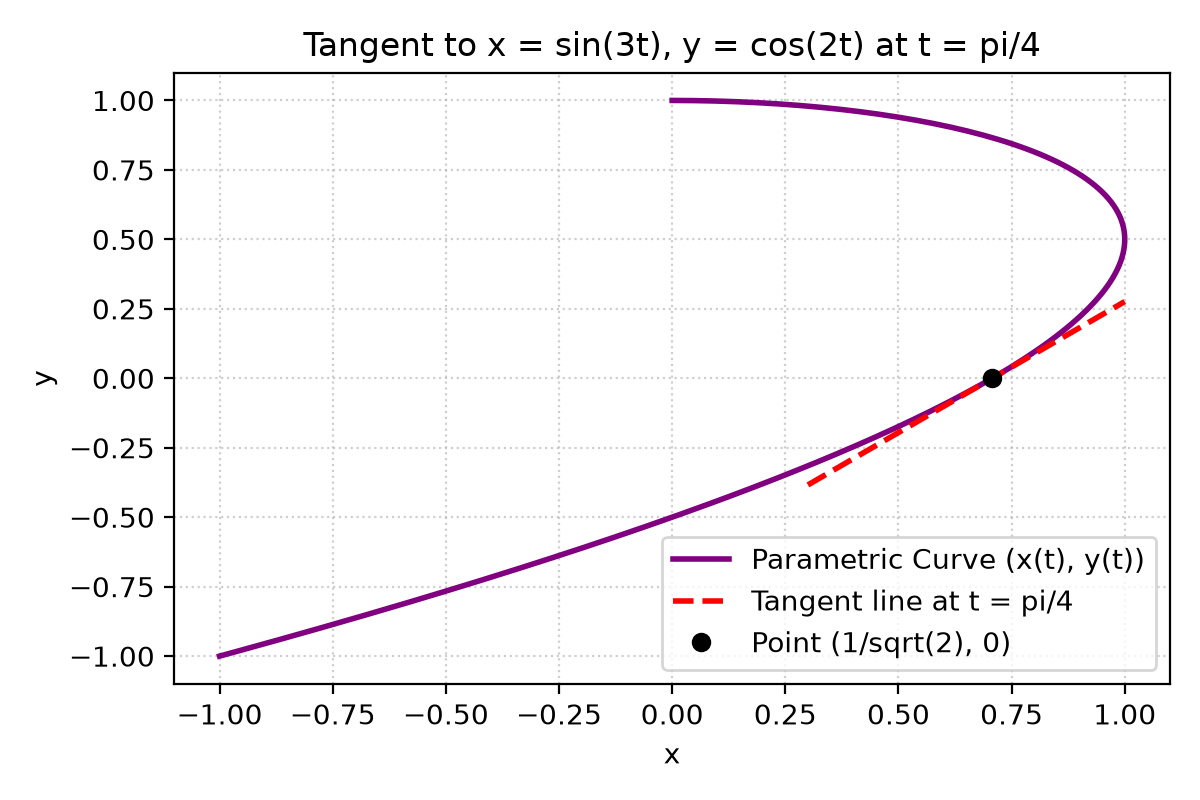
\includegraphics[width=0.65\linewidth]{figs/q16_tangent.png}
\caption{Curve $x = \sin 3t, y = \cos 2t$ and tangent line at $t = \pi/4$.}
\end{figure}
\begin{tcolorbox}[colback=gray!10,colframe=black,width=\linewidth]
\texttt{codes/q16.py}
\end{tcolorbox}

\paragraph{1.2.17 Question 17}
Evaluate:
\begin{equation}
I = \int_0^\pi \frac{x \sin x}{1 + \cos^2 x} \, dx
\end{equation}

\textbf{Solution:} Using formula \eqref{eq:def_integral_prop}:
\begin{equation}
I = \int_0^\pi \frac{(\pi - x)\sin(\pi - x)}{1 + \cos^2(\pi - x)} \, dx = \int_0^\pi \frac{(\pi - x)\sin x}{1 + \cos^2 x} \, dx
\end{equation}
Adding both equations:
\begin{align}
2I &= \pi \int_0^\pi \frac{\sin x}{1 + \cos^2 x} \, dx \\
I &= \frac{\pi}{2} \int_0^\pi \frac{\sin x}{1 + \cos^2 x} \, dx
\end{align}
Substitute $u = \cos x$, $du = -\sin x dx$. At $x = 0 \implies u = 1$; at $x = \pi \implies u = -1$:
\begin{equation}
I = \frac{\pi}{2} \int_1^{-1} \frac{-du}{1 + u^2} = \frac{\pi}{2} \int_{-1}^1 \frac{du}{1 + u^2} = \frac{\pi}{2} \left[ \tan^{-1} u \right]_{-1}^1 = \frac{\pi}{2} \left(\frac{\pi}{4} - \left(-\frac{\pi}{4}\right)\right) = \frac{\pi^2}{4}
\end{equation}
\begin{tcolorbox}[colback=gray!10,colframe=black,width=\linewidth]
\texttt{codes/q17.c}
\end{tcolorbox}

\paragraph{1.2.18 Question 18}
Solve the differential equation: $(x^2 - y^2)dx + 2xy dy = 0$ given that $y = 1$ when $x = 1$.

\textbf{Solution (via Laplace Transform):} Rewrite as:
\begin{equation}
\frac{dy}{dx} = \frac{y^2 - x^2}{2xy}
\end{equation}
Let $u = y^2 \implies \frac{du}{dx} = 2y \frac{dy}{dx}$. Thus:
\begin{equation}
x \frac{du}{dx} + u = x^2
\end{equation}
Change variable to the logarithmic domain $t = \ln x$ ($x = e^t$). With $w(t) = u(e^t)$, $\frac{du}{dx} = e^{-t} \frac{dw}{dt}$:
\begin{equation}
\frac{dw}{dt} + w = e^{2t}, \quad w(0) = y(1)^2 = 1
\end{equation}
Applying Laplace transform \eqref{eq:laplace_first_deriv} and \eqref{eq:laplace_powers}:
\begin{align}
s W(s) - w(0) + W(s) &= \frac{1}{s - 2} \\
(s + 1)W(s) &= 1 + \frac{1}{s - 2} = \frac{s - 1}{s - 2} \\
W(s) &= \frac{s - 1}{(s + 1)(s - 2)} = \frac{2/3}{s + 1} + \frac{1/3}{s - 2}
\end{align}
Taking the inverse Laplace transform:
\begin{equation}
w(t) = \frac{2}{3}e^{-t} + \frac{1}{3}e^{2t}
\end{equation}
Transforming back via $t = \ln x$:
\begin{equation}
y^2 = \frac{2}{3x} + \frac{x^2}{3} \implies 3x y^2 = 2 + x^3 \implies x^3 - 3x y^2 + 2 = 0
\end{equation}
\begin{tcolorbox}[colback=gray!10,colframe=black,width=\linewidth]
\texttt{codes/q18.py}
\end{tcolorbox}

\paragraph{1.2.19 Question 19}
Solve the differential equation: $\cos^2 x \frac{dy}{dx} + y = \tan x$.

\textbf{Solution (via Laplace Transform):} Dividing through by $\cos^2 x$:
\begin{equation}
\frac{dy}{dx} + \sec^2 x \cdot y = \tan x \sec^2 x
\end{equation}
Let $u = \tan x \implies \frac{du}{dx} = \sec^2 x$. By the chain rule, $\frac{dy}{dx} = \frac{dy}{du}\frac{du}{dx} = \sec^2 x \frac{dy}{du}$:
\begin{equation}
\frac{dy}{du} + y = u
\end{equation}
Applying Laplace transform \eqref{eq:laplace_first_deriv} with respect to $u$:
\begin{align}
s Y(s) - y(0) + Y(s) &= \frac{1}{s^2} \\
(s + 1) Y(s) &= y(0) + \frac{1}{s^2} \\
Y(s) &= \frac{y(0)}{s + 1} + \frac{1}{s^2(s+1)}
\end{align}
Using partial fractions, $\frac{1}{s^2(s+1)} = \frac{1}{s^2} - \frac{1}{s} + \frac{1}{s+1}$. Thus:
\begin{align}
Y(s) &= \frac{1}{s^2} - \frac{1}{s} + \frac{y(0) + 1}{s + 1} \\
y(u) &= u - 1 + C e^{-u}
\end{align}
where $C = y(0) + 1$. Substituting $u = \tan x$:
\begin{equation}
y(x) = \tan x - 1 + C e^{-\tan x}
\end{equation}
\begin{tcolorbox}[colback=gray!10,colframe=black,width=\linewidth]
\texttt{codes/q19.py}
\end{tcolorbox}

\paragraph{1.2.20 Question 20}
If $\mathbf{a} = \hat{i} + 4\hat{j} + 2\hat{k}$ and $\mathbf{b} = 3\hat{i} - 2\hat{j} + 7\hat{k}$, find a vector $\mathbf{c}$ such that $\mathbf{a} \times \mathbf{c} = \mathbf{b}$ and $\mathbf{a}^\top \mathbf{c} = 1$.

\textbf{Solution:} Using the vector triple product identity $\mathbf{a} \times (\mathbf{a} \times \mathbf{c}) = (\mathbf{a}^\top \mathbf{c})\mathbf{a} - \|\mathbf{a}\|^2 \mathbf{c}$:
\begin{align}
\mathbf{a} \times \mathbf{b} &= (1)\mathbf{a} - \|\mathbf{a}\|^2 \mathbf{c} \\
\|\mathbf{a}\|^2 \mathbf{c} &= \mathbf{a} - \mathbf{a} \times \mathbf{b} = \mathbf{a} + \mathbf{b} \times \mathbf{a}
\end{align}
From formula \eqref{eq:vector_norm}, $\|\mathbf{a}\|^2 = 1^2 + 4^2 + 2^2 = 21$.
\begin{equation}
\mathbf{b} \times \mathbf{a} = \begin{vmatrix} \hat{i} & \hat{j} & \hat{k} \\ 3 & -2 & 7 \\ 1 & 4 & 2 \end{vmatrix} = (-4 - 28)\hat{i} - (6 - 7)\hat{j} + (12 + 2)\hat{k} = -32\hat{i} + \hat{j} + 14\hat{k}
\end{equation}
Therefore:
\begin{equation}
\mathbf{c} = \frac{1}{21}\left[ (\hat{i} + 4\hat{j} + 2\hat{k}) + (-32\hat{i} + \hat{j} + 14\hat{k}) \right] = \frac{-31\hat{i} + 5\hat{j} + 16\hat{k}}{21}
\end{equation}
\begin{tcolorbox}[colback=gray!10,colframe=black,width=\linewidth]
\texttt{codes/q20.c}
\end{tcolorbox}

\paragraph{1.2.21 Question 21}
Find the shortest distance between the lines:
\begin{equation}
\frac{x - 3}{1} = \frac{y - 5}{-2} = \frac{z - 7}{1} \quad \text{and} \quad \frac{x + 1}{7} = \frac{y + 1}{-6} = \frac{z + 1}{1}
\end{equation}

\textbf{Solution:} Points and direction vectors are:
\begin{align}
\mathbf{a}_1 &= \begin{pmatrix} 3 \\ 5 \\ 7 \end{pmatrix}, \quad \mathbf{b}_1 = \begin{pmatrix} 1 \\ -2 \\ 1 \end{pmatrix}; \qquad \mathbf{a}_2 = \begin{pmatrix} -1 \\ -1 \\ -1 \end{pmatrix}, \quad \mathbf{b}_2 = \begin{pmatrix} 7 \\ -6 \\ 1 \end{pmatrix} \\
\mathbf{a}_2 - \mathbf{a}_1 &= \begin{pmatrix} -4 \\ -6 \\ -8 \end{pmatrix}
\end{align}
From formula \eqref{eq:cross_prod}:
\begin{equation}
\mathbf{n} = \mathbf{b}_1 \times \mathbf{b}_2 = \begin{vmatrix} \hat{i} & \hat{j} & \hat{k} \\ 1 & -2 & 1 \\ 7 & -6 & 1 \end{vmatrix} = 4\hat{i} + 6\hat{j} + 8\hat{k}
\end{equation}
By the norm procedure \eqref{eq:vector_norm}:
\begin{equation}
\|\mathbf{n}\| = \sqrt{4^2 + 6^2 + 8^2} = \sqrt{16 + 36 + 64} = \sqrt{116} = 2\sqrt{29}
\end{equation}
From formula \eqref{eq:shortest_dist}:
\begin{equation}
d = \frac{|(-4)(4) + (-6)(6) + (-8)(8)|}{2\sqrt{29}} = \frac{|-16 - 36 - 64|}{2\sqrt{29}} = \frac{116}{2\sqrt{29}} = \frac{58}{\sqrt{29}} = 2\sqrt{29}
\end{equation}
\begin{tcolorbox}[colback=gray!10,colframe=black,width=\linewidth]
\texttt{codes/q21.c}
\end{tcolorbox}

\paragraph{1.2.22 Question 22}
A pair of dice is thrown 4 times. If getting a doublet is considered a success, find the probability distribution of the number of successes.

\textbf{Solution:} When a pair of dice is rolled, the sample space has $36$ outcomes. Doublets are $\{(1,1),(2,2),(3,3),(4,4),(5,5),(6,6)\}$ (6 outcomes).
\begin{equation}
p = \frac{6}{36} = \frac{1}{6}, \quad q = 1 - p = \frac{5}{6}, \quad n = 4
\end{equation}
From Binomial distribution formula \eqref{eq:binomial}:
\begin{align}
P(X = 0) &= \binom{4}{0}\left(\frac{1}{6}\right)^0\left(\frac{5}{6}\right)^4 = \frac{625}{1296} \\
P(X = 1) &= \binom{4}{1}\left(\frac{1}{6}\right)^1\left(\frac{5}{6}\right)^3 = \frac{500}{1296} = \frac{125}{324} \\
P(X = 2) &= \binom{4}{2}\left(\frac{1}{6}\right)^2\left(\frac{5}{6}\right)^2 = \frac{150}{1296} = \frac{25}{216} \\
P(X = 3) &= \binom{4}{3}\left(\frac{1}{6}\right)^3\left(\frac{5}{6}\right)^1 = \frac{20}{1296} = \frac{5}{324} \\
P(X = 4) &= \binom{4}{4}\left(\frac{1}{6}\right)^4\left(\frac{5}{6}\right)^0 = \frac{1}{1296}
\end{align}
\begin{tcolorbox}[colback=gray!10,colframe=black,width=\linewidth]
\texttt{codes/q22.c}
\end{tcolorbox}

\newpage
\subsubsection*{Section C (6 Marks Each)}

\paragraph{1.2.23 Question 23}
Using properties of determinants, prove that:
\begin{equation}
\begin{vmatrix} \alpha & \beta & \gamma \\ \alpha^2 & \beta^2 & \gamma^2 \\ \beta+\gamma & \gamma+\alpha & \alpha+\beta \end{vmatrix} = (\beta - \gamma)(\gamma - \alpha)(\alpha - \beta)(\alpha + \beta + \gamma)
\end{equation}

\textbf{Solution:} Applying $R_3 \to R_3 + R_1$:
\begin{equation}
\Delta = \begin{vmatrix} \alpha & \beta & \gamma \\ \alpha^2 & \beta^2 & \gamma^2 \\ \alpha+\beta+\gamma & \alpha+\beta+\gamma & \alpha+\beta+\gamma \end{vmatrix} = (\alpha + \beta + \gamma)\begin{vmatrix} \alpha & \beta & \gamma \\ \alpha^2 & \beta^2 & \gamma^2 \\ 1 & 1 & 1 \end{vmatrix}
\end{equation}
Applying column operations $C_1 \to C_1 - C_2$ and $C_2 \to C_2 - C_3$:
\begin{align}
\Delta &= (\alpha + \beta + \gamma)\begin{vmatrix} \alpha - \beta & \beta - \gamma & \gamma \\ \alpha^2 - \beta^2 & \beta^2 - \gamma^2 & \gamma^2 \\ 0 & 0 & 1 \end{vmatrix} \\
&= (\alpha + \beta + \gamma)(\alpha - \beta)(\beta - \gamma) \begin{vmatrix} 1 & 1 & \gamma \\ \alpha + \beta & \beta + \gamma & \gamma^2 \\ 0 & 0 & 1 \end{vmatrix} \\
&= (\alpha + \beta + \gamma)(\alpha - \beta)(\beta - \gamma)[(\beta + \gamma) - (\alpha + \beta)] \\
&= (\alpha + \beta + \gamma)(\alpha - \beta)(\beta - \gamma)(\gamma - \alpha)
\end{align}
\begin{tcolorbox}[colback=gray!10,colframe=black,width=\linewidth]
\texttt{codes/q23.c}
\end{tcolorbox}

\paragraph{1.2.24 Question 24}
Show that the rectangle of maximum area that can be inscribed in a circle of radius $R$ is a square.

\textbf{Solution:} Let length be $2x$ and breadth be $2y$. The circle equation is $x^2 + y^2 = R^2 \implies y = \sqrt{R^2 - x^2}$.
\begin{equation}
\text{Area } A = (2x)(2y) = 4x\sqrt{R^2 - x^2}
\end{equation}
Maximizing $S = A^2 = 16(x^2 R^2 - x^4)$:
\begin{equation}
\frac{dS}{dx} = 16(2x R^2 - 4x^3) = 0 \implies 2x^2 = R^2 \implies x = \frac{R}{\sqrt{2}}
\end{equation}
Then $y = \sqrt{R^2 - \frac{R^2}{2}} = \frac{R}{\sqrt{2}}$. Furthermore, $\frac{d^2 S}{dx^2} = 16(2R^2 - 12x^2) = -64R^2 < 0$.
Since $x = y$, length = breadth = $\sqrt{2}R$. Hence, the rectangle of maximum area is a square.
\begin{tcolorbox}[colback=gray!10,colframe=black,width=\linewidth]
\texttt{codes/q24.c}
\end{tcolorbox}

\paragraph{1.2.25 Question 25}
Using integration, find the area of the region bounded by the parabola $y^2 = 4x$ and the circle $4x^2 + 4y^2 = 9$.

\textbf{Solution:} Substituting $y^2 = 4x$ into $4x^2 + 4y^2 = 9$:
\begin{equation}
4x^2 + 16x - 9 = 0 \implies (2x - 1)(2x + 9) = 0 \implies x = \frac{1}{2} \quad (x \ge 0)
\end{equation}
Due to symmetry across the $x$-axis, the total area is:
\begin{align}
A &= 2 \left[ \int_0^{1/2} 2\sqrt{x} \, dx + \int_{1/2}^{3/2} \sqrt{\frac{9}{4} - x^2} \, dx \right] \\
&= 4 \left[ \frac{2}{3}x^{3/2} \right]_0^{1/2} + 2 \left[ \frac{x}{2}\sqrt{\frac{9}{4} - x^2} + \frac{9}{8}\sin^{-1}\left(\frac{2x}{3}\right) \right]_{1/2}^{3/2} \\
&= \frac{\sqrt{2}}{6} + \frac{9\pi}{8} - \frac{9}{4}\sin^{-1}\left(\frac{1}{3}\right)
\end{align}
\begin{figure}[H]
\centering
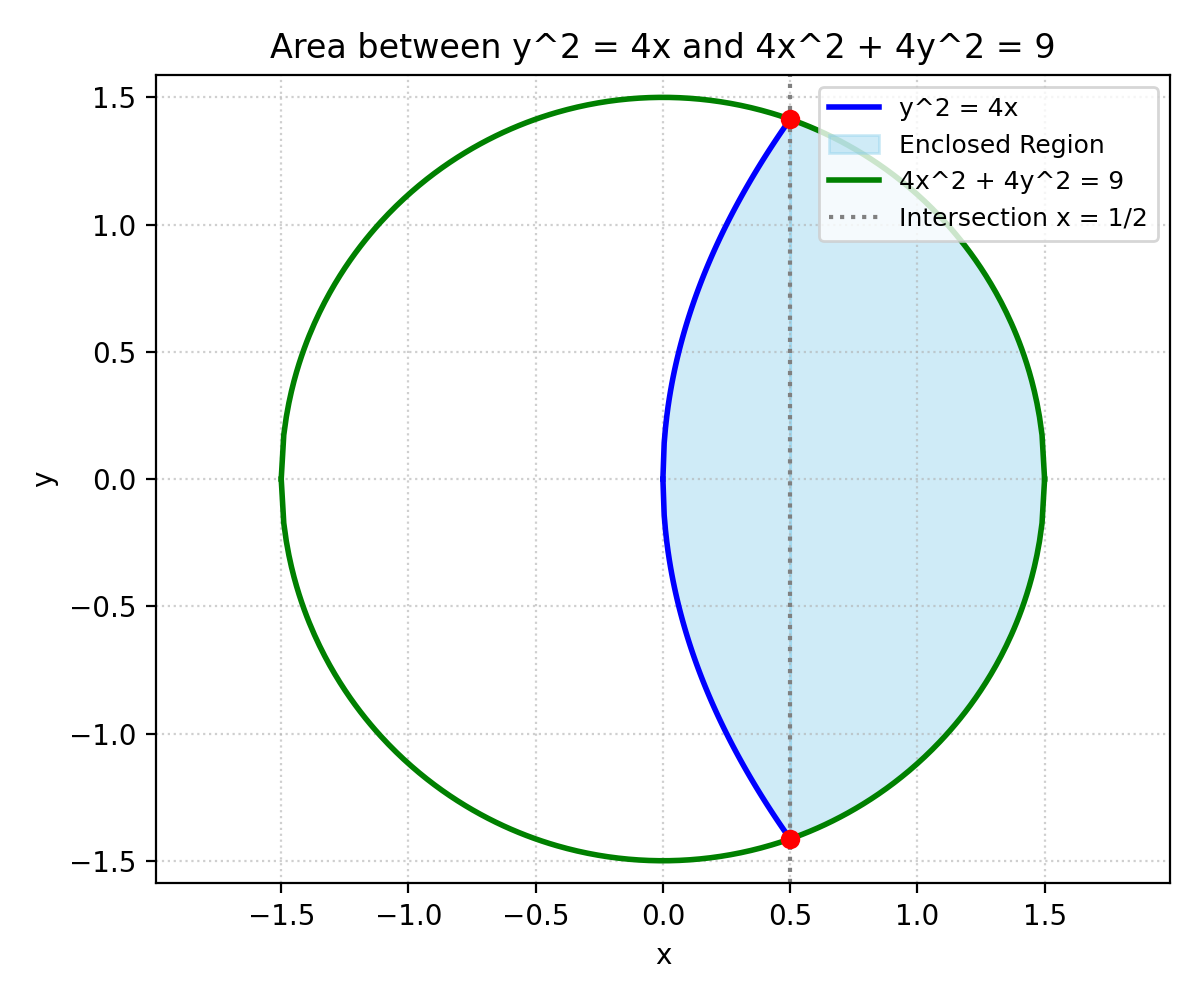
\includegraphics[width=0.65\linewidth]{figs/q25_area.png}
\caption{Region bounded by parabola $y^2 = 4x$ and circle $4x^2 + 4y^2 = 9$.}
\end{figure}
\begin{tcolorbox}[colback=gray!10,colframe=black,width=\linewidth]
\texttt{codes/q25.py}
\end{tcolorbox}

\paragraph{1.2.26 Question 26}
Evaluate:
\begin{equation}
I = \int_{-a}^a \sqrt{\frac{a - x}{a + x}} \, dx
\end{equation}

\textbf{Solution:} Rationalizing the numerator:
\begin{equation}
I = \int_{-a}^a \frac{a - x}{\sqrt{a^2 - x^2}} \, dx = a \int_{-a}^a \frac{dx}{\sqrt{a^2 - x^2}} - \int_{-a}^a \frac{x}{\sqrt{a^2 - x^2}} \, dx
\end{equation}
The second integral has an odd integrand over $[-a, a]$, so it evaluates to $0$. The first integrand is even:
\begin{equation}
I = 2a \int_0^a \frac{dx}{\sqrt{a^2 - x^2}} = 2a \left[ \sin^{-1}\left(\frac{x}{a}\right) \right]_0^a = 2a\left(\frac{\pi}{2} - 0\right) = \pi a
\end{equation}
\begin{tcolorbox}[colback=gray!10,colframe=black,width=\linewidth]
\texttt{codes/q26.c}
\end{tcolorbox}

\paragraph{1.2.27 Question 27}
Find the equation of the plane passing through $(-1, -1, 2)$ and perpendicular to the planes $2x + 3y - 3z = 2$ and $5x - 4y + z = 6$.

\textbf{Solution:} Normal vectors to the given planes are $\mathbf{n}_1 = \begin{pmatrix} 2 \\ 3 \\ -3 \end{pmatrix}$ and $\mathbf{n}_2 = \begin{pmatrix} 5 \\ -4 \\ 1 \end{pmatrix}$.
The normal $\mathbf{n}$ to the required plane is:
\begin{equation}
\mathbf{n} = \mathbf{n}_1 \times \mathbf{n}_2 = \begin{vmatrix} \hat{i} & \hat{j} & \hat{k} \\ 2 & 3 & -3 \\ 5 & -4 & 1 \end{vmatrix} = -9\hat{i} - 17\hat{j} - 23\hat{k}
\end{equation}
Using point-normal form with point $\mathbf{x}_0 = (-1, -1, 2)^\top$:
\begin{align}
-9(x + 1) - 17(y + 1) - 23(z - 2) &= 0 \\
-9x - 17y - 23z - 9 - 17 + 46 &= 0 \\
9x + 17y + 23z &= 20
\end{align}
\begin{tcolorbox}[colback=gray!10,colframe=black,width=\linewidth]
\texttt{codes/q27.c}
\end{tcolorbox}

\paragraph{1.2.28 Question 28}
A factory owner purchases machines A and B. Area occupied: A needs $1000\,\text{m}^2$, B needs $1200\,\text{m}^2$ (Max $9000\,\text{m}^2$). Labour required: A needs $12$ men, B needs $8$ men (Max $72$ men). Daily output: A produces $60$, B produces $40$. How many machines of each type maximize daily output?

\textbf{Solution:} Let $x$ be the number of machine A and $y$ be the number of machine B.
\begin{align}
\text{Maximize } & Z = 60x + 40y \\
\text{Subject to } & 1000x + 1200y \le 9000 \implies 5x + 6y \le 45 \\
& 12x + 8y \le 72 \implies 3x + 2y \le 18 \\
& x, y \ge 0, \quad x, y \in \mathbb{Z}_{\ge 0}
\end{align}
The corner points of the feasible region are:
\begin{itemize}
    \item $(0, 0) \implies Z = 0$
    \item $(6, 0) \implies Z = 60(6) + 40(0) = 360$
    \item $(0, 7) \implies Z = 60(0) + 40(7) = 280$
    \item Feasible integer points near the boundary: $(2, 5) \implies 3(2)+2(5)=16 \le 18$, $5(2)+6(5)=40 \le 45 \implies Z = 120 + 200 = 320$.
\end{itemize}
Maximum daily output is $360$ units, achieved by purchasing $6$ machines of type A and $0$ machines of type B.
\begin{figure}[H]
\centering
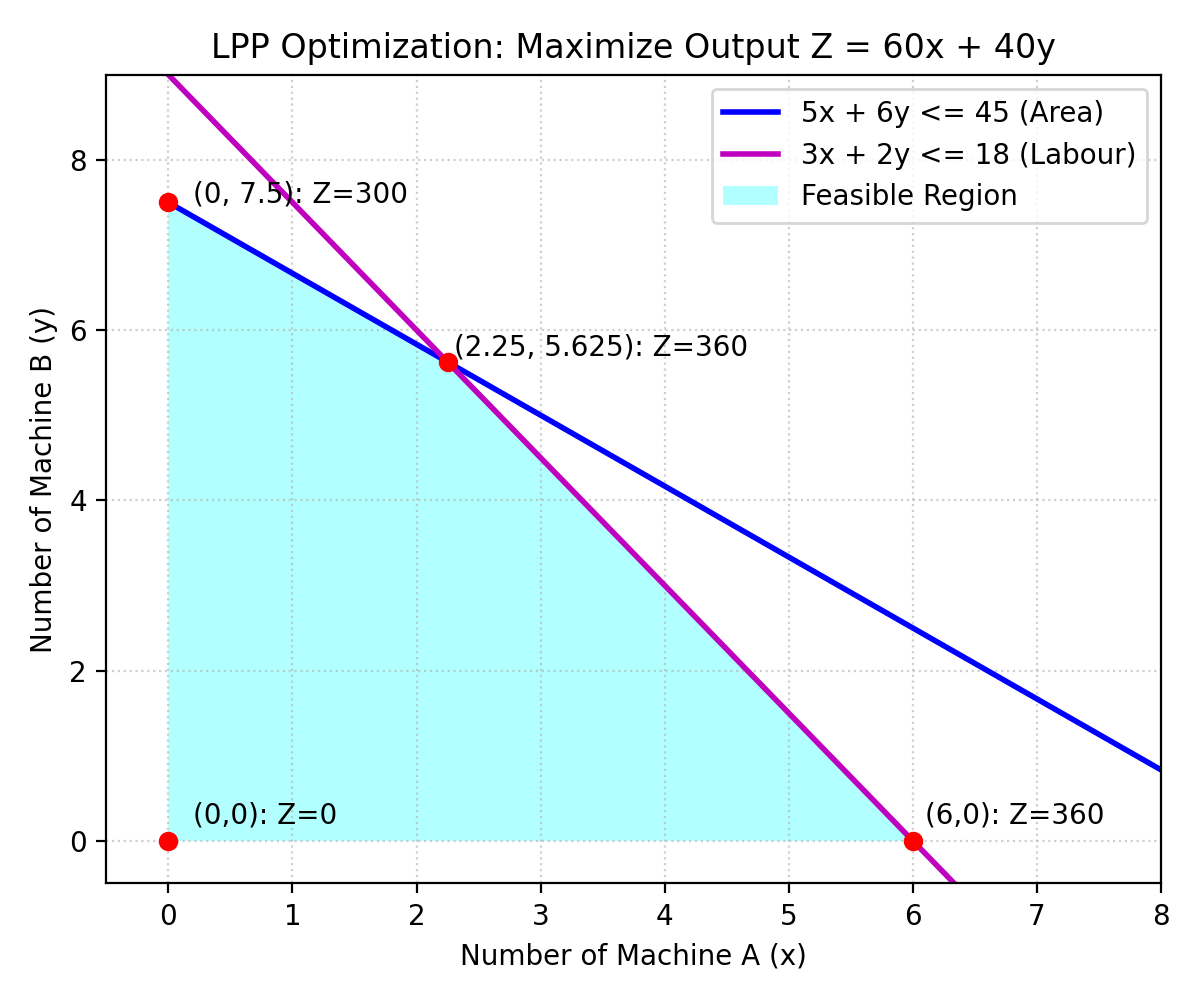
\includegraphics[width=0.65\linewidth]{figs/q28_lpp.png}
\caption{Feasible region and optimal corner point for machine allocation.}
\end{figure}
\begin{tcolorbox}[colback=gray!10,colframe=black,width=\linewidth]
\texttt{codes/q28.py}
\end{tcolorbox}

\paragraph{1.2.29 Question 29}
An insurance company insured 2000 scooter drivers, 4000 car drivers, and 6000 truck drivers. Probability of accident: scooter = $0.01$, car = $0.03$, truck = $0.15$. An insured person meets with an accident. What is the probability that he is a scooter driver?

\textbf{Solution:} Total insured drivers $= 2000 + 4000 + 6000 = 12000$.
Let $E_1, E_2, E_3$ be the events of selecting scooter, car, and truck drivers respectively, and $A$ be the event of an accident:
\begin{align}
\Pr(E_1) &= \frac{2000}{12000} = \frac{1}{6}, \quad \Pr(A|E_1) = 0.01 = \frac{1}{100} \\
\Pr(E_2) &= \frac{4000}{12000} = \frac{1}{3}, \quad \Pr(A|E_2) = 0.03 = \frac{3}{100} \\
\Pr(E_3) &= \frac{6000}{12000} = \frac{1}{2}, \quad \Pr(A|E_3) = 0.15 = \frac{15}{100}
\end{align}
Applying Bayes' Theorem \eqref{eq:bayes}:
\begin{align}
\Pr(E_1|A) &= \frac{\Pr(E_1)\Pr(A|E_1)}{\Pr(E_1)\Pr(A|E_1) + \Pr(E_2)\Pr(A|E_2) + \Pr(E_3)\Pr(A|E_3)} \\
&= \frac{\frac{1}{6} \times \frac{1}{100}}{\frac{1}{6} \times \frac{1}{100} + \frac{1}{3} \times \frac{3}{100} + \frac{1}{2} \times \frac{15}{100}} \\
&= \frac{\frac{1}{6}}{\frac{1}{6} + 1 + \frac{15}{2}} = \frac{\frac{1}{6}}{\frac{1 + 6 + 45}{6}} = \frac{1}{52}
\end{align}
\begin{tcolorbox}[colback=gray!10,colframe=black,width=\linewidth]
\texttt{codes/q29.c}
\end{tcolorbox}

\end{document}
